\documentclass[12pt]{article}

\usepackage{amsthm}
\usepackage{amsmath}
\usepackage{graphicx}





% collectivised from: https://www.overleaf.com/learn/latex/Theorems_and_proofs#Theorem_styles
\theoremstyle{definition}
\newtheorem{definition}{Definition}[section]

\theoremstyle{remark}
\newtheorem*{remark}{Remark}
\newtheorem{theorem}{Theorem}[section]
\newtheorem{lemma}[theorem]{Lemma}
%
\begin{document}
%Plan
%   1. Introduction
%       Original problem: US graphs and edge coloration with \omega = 2. 
%       Known for delta 2. we know delta is at most 5. Concept of direction.
%   2. On a grid    
%       "what we will do here: ... ". RK: if not all on a grid are US, all US are on a grid. Thus any result on on a grid graph is true for US. 
%       2.1 On a grid - definition. 
%       2.2 Additional concepts: Type 1/2 diagonals, order on the diagonals.
%       2.3 Algorithm 
%       2.4 Complexity
%   3. Applications
%       3.1 US graphs: chromatic index of 4
%       3.2 angles & directions
\section{Introduction}
The original problem is to study the chromatic index of triangle-free \textit{unit square intersection graphs},
which are graphs that are obtained for a family of unit squares. 
Each square is represented by a vertex in a graph, and each edge represent the fact that two squares are intersecting. \\
We already know that when the maximum degree $\Delta$ is $2$, there may exists graphs of type 2, for instance any odd cycle. We can also observe that
when two unit squares intersects, there is a corner of each inside the other; from this observation follows that there cannot be 
a triangle-free unit square graph with $\Delta \ge 5$. \\
In what follows, we provide a proof that there cannot be a graph of type 2 when $\Delta = 4$. The proof will be done by introducing a new way to
represent the graphs by using a grid; and we will call them \textit{on a grid} graphs.

\section{Graphs on-a-grid}
We present in this section a proof that unit square graphs are also \textit{on a grid} graphs. 
\subsection{On a grid}
\begin{definition}[On a grid]
    A graph is said \textit{on a grid} if:
    \begin{itemize}
        \item All the edges are either parallels or perpendicular.
        \item All the edges are of integer lengths.
        \item No edge is overlapping or containing an other edge in more than one point.
    \end{itemize}
\end{definition}

Instead of using the usual directions of the cartesian plane, we will rotate all the edges by $\tfrac{\pi}{4}$ as it will be more convenient later.
The graph represented in Fig.1. is \textit{on a grid}.

\begin{figure}[h]
    \centering
    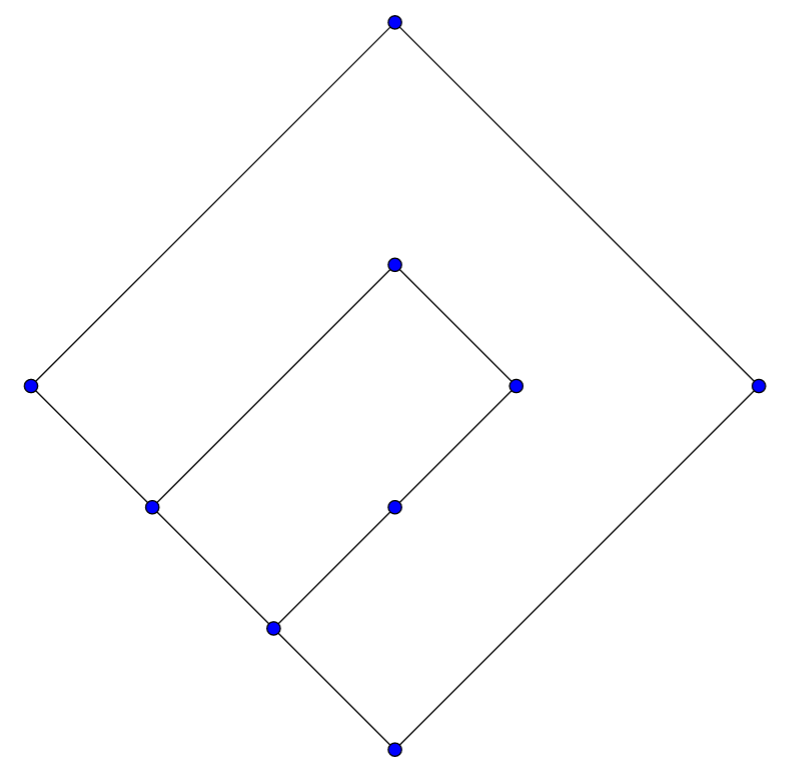
\includegraphics[scale=0.2]{tex_images/on_a_grid_g1.png}
    \caption{$G_1$ is on a grid.}
\end{figure}

\begin{remark}
    $G_1$ has exactly $10$ edges.
\end{remark}

\subsection{Additional concepts}

\begin{definition}[Direction of intersection]
    Let $a, b$ be two unit squares. We say that $a$ intersects $b$ in UR direction (resp. UL, DL, DR) if the up-right (resp up-left, down-left, down-right) corner
    of $a$ is inside $b$.     
\end{definition}

\begin{figure}[h]
    \centering
    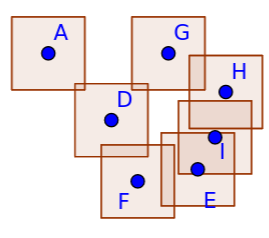
\includegraphics[scale = 0.3]{tex_images/same_diagonals.png}
    \caption{Illustration of direction of intersections.}
\end{figure}

For instance, in Fig. 2, $D$ intersect $F$ in direction DR, $G$ in direction UR and $A$ in direction UL. Conversely, $A$ intersect $D$ in direction DR.

\begin{lemma}
    If $a$ intersect both $b$ and $c$ in the same direction, then $a, b$ and $c$ forms a triangle.
\end{lemma}

\begin{proof}
    Notice that they would all share a common point in a certain corner of $a$.
\end{proof}

\begin{definition}[Diagonals]
    Let $a$ and $b$ be two squares. They are said to be on the same \textit{Type 1 diagonal} (resp. Type 2) if you can find a sequence $\{s_1, ... s_k\}$ of squares such that:
    \begin{itemize}
        \item $s_1 = a$
        \item $s_k = b$
        \item $\forall i \in \{1, .. , k-1\}$, $s_i$ intersects $s_{i+1}$ in UL or DR (resp. UR or DL) direction.
    \end{itemize}    
    A diagonal is a set of points (possibly trivial) that are on the same diagonal. 
\end{definition}

\begin{remark}
    We will denote the diagonal as follows : $D:= \{d_1, ... , d_k\}$. In this case $d_1$ is the highest square of the diagonal, meaning that $d_1$ intersect $d_2$ in DR direction in the case of a type 1 diagonal, and so on.
\end{remark}

In Fig. 2 we can denote the following diagonals:\\
Type 1: $\{(A, D, F), (E), (I), (G, H)\}$\\
Type 2: $\{(A), (D,G), (F, E, I, H)\}$\\


\begin{lemma}
    Let $D$, $E$ be two diagonals of the same type. If we can find $d \in D$; $e \in E$ such that $d$ intersect $e$ in some direction X, then: \\\
    $\forall d' \in D$, $\forall e' \in E$, either $e'\cap d' = \emptyset$ or $d'$ intersect $e'$ in direction X.
\end{lemma}

\begin{proof}
    Without loss of generality, let $D:=\{d_1, ... d_k\}$ and $E:= \{e_1, ... e_l\}$ be two distinct diagonals of Type 1. 
    Suppose $d_1$ intersect $e_1$ in direction DL. \\
    Let $(i,j)$ be the smallest couple different from $(1,1)$ such that $d_i \cap e_j \ne \emptyset$. Observe that as $D$ and $E$ are Type 1, the only possibility is that 
    $d_i$ intersect $e_j$ in direction UR or DL.
\end{proof}

We can now use the previous lemma to define a partial order on our diagonals.

\begin{definition}[Order on diagonals]
    Let $D_1$, $D_2$ two diagonals of Type 1 (resp Type 2). We say that $D_1$ is \textit{directly higher} than $D_2$, or $D_1 >_d D_2$ if:
    $\exists d_1 \in D_1, \exists d_2 \in D_2$ such that $d_1$ intersects $d_2$ in DL (resp. UR) direction. \\ \\
    We say that $D_1$ is higher than $D_2$, or $D_1 > D_2$ if we can find a sequence of diagonals $\{s_1, ... , s_k\}$ such that:
    \begin{itemize}
        \item $s_1 = D_1$
        \item $s_k = D_2$
        \item $\forall i \in \{1, ..., k-1\}, s_i >_d s_{i+1}$
    \end{itemize} 
\end{definition}

%% TODO: explain why we cant have D >_d E and E >_d D at the same time 

\begin{remark}
    Note that $>_d$ is not an order as it is not transitive. 
\end{remark}


\subsection{From unit squares to the grid}

We present here an algorithm to obtain a on a grid graph given a family of unit squares.\\
Start by identifying all the diagonals: to do so,

\section{Some applications}
\subsection{Edge coloration}

One can easily see that any on a grid graph has a chromatic index of at most $4$. As every triangle-free unit square graph is also on a grid, 
it follows that no graph of type 2 can exist for these if $\Delta = 4$.

\begin{theorem}
    Let $G$ be a unit square graph, with $\Delta = 4$ and $\omega = 2$. Then $\chi'(G) = 4$.
\end{theorem}

\begin{proof}
    It is sufficient to show it is true for all graphs that are on a grid. \\
    Let $G$ be on a grid. Delete for a moment all the edges that correspond to type 1 diagonals. There subsits only paths. 
    As all paths can be colored using only two colors, assign color 1 or 2 to all the remaining edges. \\
    Do the same thing for the type 2 diagonals with colors 3 and 4. \\
    As all the edges of $G$ are either on a type 1 or a type 2 diagonal, all the edges are assigned to a color. If two edges are on the same type of diagonals, either they
    have different colors or they are not adjacent. If two edges are on different type of diagonals, they have different colors. Therefore, this coloration is acceptable.
\end{proof}

\subsection{Directions in cycles}


\end{document}